\documentclass[
	%parspace, % Add vertical space between paragraphs
	%noindent, % No indentation of first lines in each paragraph
	%nohyp, % No hyphenation of words
	%twoside, % Double sided format
	%draft, % Quicker draft compilation without rendering images
	%final, % Set final to hide todos
]{elteikthesis}[2024/04/26]

% The minted package is also supported for source highlighting
% See elteikthesis_minted.tex for example
%\usepackage[newfloat]{minted}

% Document's metadata
\title{Data-Driven Object-Centric Simulation for Airport Turnaround Analysis and Resource Optimization} % title
\date{2026} % year of defense

% Author's metadata
\author{Amir Abdelsayed}
\degree{Data Science MSc}

% Superivsor(s)' metadata
\supervisor{István Koren} % internal supervisor's name
\affiliation{Head of Department} % internal supervisor's affiliation
%\extsupervisor{Jane Doe} % external supervisor's name
%\extaffiliation{Senior Developer} % external supervisor's affiliation

% University's metadata
\university{Eötvös Loránd University} % university's name
\faculty{Faculty of Informatics} % faculty's name
\department{Dept. of Software Technology and Methodology} % department's name
\city{Budapest} % city
\logo{elte_cimer_szines} % logo

% Add bibliography file
\addbibresource{study_references.bib}

% The document

\begin{document}
\documentlang{english}
\maketitle
\chapter*{Abstract}
\addcontentsline{toc}{chapter}{Abstract}
Detailed records of airport ground services are often unavailable, although turnaround performance depends on their timing and shared resources. This thesis investigates how limited Berlin Brandenburg Airport observations can support an object-centric turnaround simulation. We adapt an existing OCPN airport model, prepare aircraft-linked demand and export generated events for analysis in Promenade. Observed inputs are kept separate from literature-based service timings and other assumptions. The analysis examines resource waiting, parallel completion and the interpretation of object-centric executions. A controlled pilot compares six scenarios on two dates, with five independent runs per scenario and date. All 60 runs complete, producing 15,270 simulated executions from 509 reused empirical interval cases. With inherited curfew disabled, literature timing assumptions reduce mean simulated block duration by 7.53 and 7.04 minutes compared with the original service functions. Increasing fuel capacity substantially reduces dispatch waiting, while its effect on final turnaround is much smaller. The results also reveal an interaction between service timing and inherited policy, including a confirmed UTC/local-time mismatch. These findings support conditional analysis of the adapted model. Missing internal service observations, long stays and assumed operational context limit conclusions about actual BER performance. Further empirical evaluation is required before claiming validated calibration or optimal resource allocation.
\cleardoublepage
\tableofcontents
\cleardoublepage
\chapter{Introduction}
\label{ch:intro}

Aircraft turnaround is the period between an aircraft's arrival at a parking position and its departure for the next flight. During this period, several teams prepare the aircraft by unloading baggage, cleaning the cabin, refueling and boarding passengers. These activities follow different dependencies. Some can take place at the same time, while others can start only after preceding work has finished. Aircraft also share stands, service vehicles and ground teams. As a result, the availability of one resource can affect several turnarounds.

Understanding these interactions requires information about both the activities and the resources involved. However, the available operational records do not describe every ground service. They mainly provide information about flight movements and selected departure milestones. This creates a gap between the process we want to study and the behavior we can directly observe.

This thesis investigates how an object-centric simulation can support turnaround analysis under these conditions. We adapt an existing airport model using prepared observations from Berlin Brandenburg Airport (BER), document the assumptions used for missing information and analyze the generated event logs. We then compare service-time assumptions, policy rules and resource capacities through repeated simulation. The reported results concern the completed pilot study. Further empirical evaluation is required before the model can support conclusions about actual BER performance.

\section{Background}
Airport Collaborative Decision Making (A-CDM) supports information exchange among airport partners and the Network Manager, with particular attention to turnaround and pre-departure processes \cite{eurocontrol_acdm}. This information helps partners coordinate their activities. Nevertheless, an A-CDM-related application does not necessarily provide the start and end times of every ground service. A time interval between two milestones may contain several activities, waiting and parking. Its total duration is therefore insufficient to determine how long each internal activity took.

Object-centric event logs provide a way to retain the relationships between these activities and the objects involved. An event can be linked to a turnaround, an aircraft and a service resource. OCEL 2.0 supports these relationships, their qualifiers and changes in object attributes \cite{ocel2}. This is useful when a cleaning team or a fueling vehicle serves several aircraft during the same day.

The simulation used in this thesis is based on the \emph{Airport Ground Handling (Extended)} model provided by the supervisor, Istv\'an Koren, in OCPN Studio \cite{ocpn_studio}. Its original process structure and resource logic are retained as attributed prior work. Our modifications concern the empirical demand, aircraft pairing, selected activity timings, analysis procedures and controlled experiments.

\section{Motivation}
A departure time alone does not explain why an aircraft was ready late. The aircraft may have been waiting for a resource, receiving a service or waiting for another parallel activity to finish. These explanations require different operational responses. For example, increasing the number of fueling units can reduce the fuel queue without substantially shortening turnaround if boarding is still in progress.

Simulation allows us to examine these relationships under defined conditions. It also allows assumptions to be changed individually while keeping other inputs fixed. However, the resulting events remain synthetic. Their detail must not be mistaken for additional observations of real ground handling. The motivation of this study is therefore twofold: to investigate dependencies within the model and to make clear which conclusions the available evidence supports.

\section{Problem Statement}
The research objective is to use A-CDM information to support the calibration of an object-centric turnaround simulation and the evaluation of resource allocation. The collected data do not contain reliable internal service start/end times or measured block times. The implemented study therefore combines OpenSky flight-boundary observations with A-CDM reference records. Literature and explicitly stated assumptions supply the missing service inputs.

The problem is to construct an executable and traceable model from these sources without treating assumed durations as measured values. A second challenge is to interpret its outputs correctly. Changes in simulated turnaround may result from service timing, resource availability or policy logic. These effects must be examined separately before drawing conclusions about calibration or allocation.

\section{Research Questions}
The following research questions guide the study:
\begin{description}
\item[RQ1:] How can A-CDM Data be used to calibrate activity durations and temporal dependencies in an OCPN Simulation?
\item[RQ2:] How do dependencies between aircraft, stands, and shared ground-service resources contribute to waiting times and delay propagation at terminal stands and remote stands in an OCPN simulation?
\item[RQ3:] How can the calibrated simulation be used to evaluate resource-allocation strategies and identify configurations that reduce turnaround delays and resource contention?
\end{description}

The current work addresses these questions to different extents. For RQ1, we examine which model inputs can be supported by the collected data. For RQ2, we analyze resource waiting and the synchronization of parallel activities. A controlled comparison of terminal and remote stands, and a quantified analysis of delay propagation between flights, remain open. For RQ3, we evaluate selected capacity changes under fixed assumptions. Predictive accuracy is relevant to the evaluation of the model as a whole; it does not replace the dependency-focused meaning of RQ2.

\section{Research Goals and Contributions}
The study aims to prepare aircraft-linked input records, adapt the existing model, export analyzable object-centric logs and compare selected scenarios. The completed contributions are:
\begin{enumerate}
\item A preparation procedure that retains source references, candidate aircraft pairings and the meaning of each timestamp.
\item Daily OCPN models with finite empirical demand and persistent aircraft identities, with observed inputs separated from assumptions.
\item An analysis of the exported logs in Promenade, including resource queues, parallel completion and the effect of case definitions.
\item A controlled pilot of 60 simulation runs examining service timing, inherited policy and resource capacity.
\end{enumerate}

These contributions extend the use and evaluation of the supplied model. They do not include the development of its original six-thread process structure. Nor do they establish a validated BER digital twin or an optimal staffing plan.

\section{Thesis Structure}
Chapter~\ref{ch:related} reviews the methodological background and related work. Chapter~\ref{ch:methods} describes the data, model changes and experimental procedure. Chapter~\ref{ch:results} presents the Promenade analysis and repeated simulation results. Chapter~\ref{ch:discussion} relates the findings to the research questions and discusses their limitations. Finally, Chapter~\ref{ch:conclusion} summarizes the work and identifies the next evaluation steps.

\cleardoublepage
\chapter{Related Work and Methodological Background}
\label{ch:related}

This chapter introduces the work used to guide the study. We first consider turnaround timing and the available operational observations. We then discuss object-centric simulation and a closely related trace-reconstruction thesis. The final section explains the position of the present work.

\section{Turnaround Dependencies and Activity Timing}
Schultz et al. describe stochastic turnaround processes and discuss how disturbances on a critical path can affect later operations \cite{schultz2012dynamic}. Their work supports a model in which concurrent services must synchronize before the aircraft can proceed. It also provides reference assumptions used here for narrowbody cleaning, fueling and boarding.

Transferring a reference distribution does not establish that it describes BER operations. In this study, the distributions are used as stated model inputs. We do not estimate them from the Berlin boundary intervals or derive a universal timing difference between low-cost and full-service airlines.

Schultz later presents a calibrated stochastic boarding model and evaluates boarding scenarios \cite{schultz2018boarding}. This work shows the importance of considering passenger boarding in turnaround analysis. Our implementation uses a passenger-dependent mean reference, rather than reproducing that detailed stochastic model or its validation.

\section{Operational Observations and the Data Gap}
EUROCONTROL describes A-CDM as an approach for sharing operational information among airport operators, aircraft operators, ground handlers, air traffic control and the Network Manager \cite{eurocontrol_acdm}. This provides the operational context for milestone analysis. Whether a particular collection contains enough detail for activity-level calibration must still be checked separately.

The OpenSky REST API provides aircraft identifiers, first and last observation timestamps, and estimated airports for flight records \cite{opensky_rest}. These fields support candidate aircraft pairing. However, they do not directly measure arrival at or departure from a stand. Accordingly, the observed boundary interval and the simulated block duration are treated as different quantities throughout this thesis.

\section{Object-Centric Simulation and Event Logs}
OCEL 2.0 represents events, objects, attributes and their relationships \cite{ocel2}. We use this representation to retain the links between generated turnaround events and reusable resources. Promenade provides exploratory views of these logs and their temporal behavior \cite{promenade}. These views help explain the simulation output, but cannot independently confirm that its input assumptions are realistic.

OCPN Studio provides the modeling environment and the extended airport example \cite{ocpn_studio}. The official CPNsim runtime executes colored Petri nets \cite{cpnsim}. Our runs use its installed WebAssembly version 0.6.2. These software references document the implementation environment; they are not empirical evidence about airport operations.

\section{Turnaround Trace Reconstruction from Sparse Data}
Tkacenko's bachelor thesis investigates the generation of detailed turnaround traces when only limited observations are available \cite{tkacenko2026}. The study models narrowbody operations at Frankfurt Airport in \texttt{cpn-py}, combines domain knowledge with duration assumptions and exports simulated traces as OCEL 2.0. Candidate traces are filtered using observed in-block and off-block boundaries. The evaluation distinguishes model completion properties, empirical activity-duration agreement and relational checks on the exported data.

This work is relevant because it makes a distinction that also matters here: agreement with a total turnaround duration does not establish that the internal activity durations are correct \cite[Sections~6.2 and~7.4]{tkacenko2026}. The accepted traces in that study show different levels of agreement across activities. This supports the need to report the limits of reconstruction from sparse observations.

The present study follows a different evaluation procedure. We release demand using OpenSky observation boundaries and retain A-CDM records as references. We do not filter simulation runs to make them fit observed off-block times. Instead, we compare timing, policy and capacity assumptions under the same daily demand. The resulting differences describe the behavior of the adapted model. They do not establish that the missing Berlin service events have been accurately reconstructed.

The uncertainty measures also serve different purposes. Tkacenko compares individual ground-truth activity durations with central empirical intervals of simulated durations. Our controlled experiment calculates confidence intervals for differences between replication-level means. An interval describing activity variation is therefore not interchangeable with an interval describing uncertainty in a mean comparison.

\section{Position of the Present Study}
The contribution of this work is the connection of a traceable Berlin demand cohort to the supplied extended model, followed by object-centric analysis and repeated scenario comparisons. We attribute the original airport process model to the supervisor and cite Tkacenko's thesis as related methodological work. The two implementations are not assumed to be identical.

The completed study does not include a JFK evaluation, a replication of a particular LAX study, a trained machine-learning duration predictor or empirical conformance checking. These remain outside the results reported here.

\section{Summary}
The reviewed work provides a basis for modeling parallel services and analyzing synthetic object-centric logs. It also shows why sparse operational timestamps cannot by themselves validate internal activities. The following chapter explains how these considerations guide our input preparation and experimental design.

\cleardoublepage
\chapter{Data and Simulation Methodology}
\label{ch:methods}

This chapter describes how the available observations are converted into simulation inputs. We first define the data sources and the daily cohorts. We then explain the changes to the supplied model, the service-time assumptions and the OCEL export. Finally, we present the controlled experiment, its metrics and the technical checks. The procedure keeps observed values, literature inputs and generated events separate.

\section{Data provenance and cohort construction}
The prepared OpenSky movement table contains 22,635 records: 11,316 arrivals and 11,319 departures. Candidate BER ground intervals link an observed arrival to the following observed BER departure of the same ICAO24 identifier. The prepared core cohort contains 10,940 interval rows: 8,951 in the 15-minute to six-hour band and 1,989 in the six-to-24-hour band. Each row represents a candidate aircraft-linked interval, not a certified aircraft rotation.

The intended collection begins on 1 October 2026. The core file also includes 54 arrivals on 30 September paired to departures entering the requested period. Arrival observations in the file extend through 9 November. Accordingly, this version does not claim complete data coverage through 13 November. Temporal coverage, API availability and filtering must be distinguished from the number of interval rows retained.

We use the term boundary proxy for the interval between the last observation of the inbound flight and the first observation of the outbound flight. For case $i$, this interval is defined as
\begin{equation}
G_i^{\mathrm{proxy}}=t_{i,\mathrm{outbound\ firstSeen}}-t_{i,\mathrm{inbound\ lastSeen}}.
\end{equation}
Both timestamps are observation boundaries, as described by the OpenSky API \cite{opensky_rest}. The interval may include unobserved approach/taxi segments, parking and timetable buffers. It is not measured actual in-block time (AIBT) to actual off-block time (AOBT). Source identifiers, pairing basis, review flags and timezone-aware UTC/Berlin representations are retained.

A-CDM reference records provide candidate aircraft/airline/stand context and departure-time cross-checks where a candidate match exists. Their naive timestamps are retained alongside the UTC timezone hypothesis used during reconciliation. They are references rather than complete service-event ground truth. Credentials and API secrets are not included in the thesis or its analysis artifacts.

\section{Daily experimental inputs}
The daily models use 271 cases and 235 distinct aircraft on 1 November, and 238 cases and 212 aircraft on 8 November. Supported candidate aircraft types exist for 216 and 180 input rows, respectively. This row-level coverage does not mean every final aircraft configuration is observed: the first case establishes a persistent model configuration, and missing or unsupported types fall back to an assumed A320 configuration. Later conflicting candidates have not been reconciled.

The two cohorts include 39 and 44 intervals longer than six hours. A long interval may include parking or a timetable buffer rather than continuous ground handling. In addition, movements without an accepted pair are excluded. The simulated queues therefore describe competition within the selected cohort. They cannot be interpreted as queues caused by all BER traffic.

\section{Baseline attribution and study modifications}
The supervisor's original extended model is preserved unchanged. Its six parallel handling threads, resource interaction logic, vehicle positions, fuel supply mechanisms and process dependencies are inherited contributions. A same-demand original-timing comparator retains the original service functions within the adapted demand model; it is not the untouched example.

We replace the original continuous generation of synthetic flights with a finite set of timed arrivals. Each case is released using its observed arrival boundary proxy. The paired arrival and departure require the same aircraft identity, which becomes available again after simulated takeoff. If a later case requires that aircraft while it is still in the model, the case must wait. Synthetic outstation travel and the inherited inbound curfew/extra approach delay are bypassed; landing roll, runway contention and taxi-in remain simulated. Observed outbound times are retained outside the model as evaluation references and do not force simulated departures.

Schengen stand segregation is disabled because route context is incomplete; physical size compatibility remains. Departure-planning steps are labeled as assumptions rather than observed TOBT/TSAT values. Simulated weather, remaining durations and illustrative geometry are retained as assumptions.

\section{Service-time assumptions}
For narrowbody aircraft, the transferred reference functions, in minutes, are \cite{schultz2012dynamic}:
\begin{align}
D_{\mathrm{clean}} &=5+\mathrm{Weibull}(\mathrm{shape}=2.16,\mathrm{scale}=6.76),\\
D_{\mathrm{fuel}} &=2+\mathrm{Gamma}(\mathrm{shape}=1.64,\mathrm{scale}=9.12),\\
D_{\mathrm{board}} &=2.3+0.075P,
\end{align}
where $P$ is the assumed passenger count. Boarding uses a deterministic mean reference, not a full distribution. Vehicle travel/access time is additional where specified by the inherited model. The order of distribution arguments is checked against the runtime implementation. Its functions take scale before shape, so the calls are \texttt{weibull(6.76,2.16)} and \texttt{gamma(9.12,1.64)} before converting minutes to milliseconds. Other aircraft-size categories retain inherited timing functions.

Passenger counts are assumed at 85\% of scenario seating capacity, PRM demand is zero, and sector duration is 120 minutes. Carrier class remains unknown. No measured passenger load or justified budget/full-service timing coefficient is available. The original timing comparator's unknown-carrier branch also needs to be considered when interpreting the comparison.

The inherited 25-stand geometry, runway dimensions, resource capacities, taxi assumptions and optional-service probabilities are not verified BER infrastructure. Models begin each daily run with free stands and resources, without calibrated overnight occupancy or a warm-up history. These choices restrict interpretation of queues and resource experiments.

\section{OCEL export and Promenade procedure}
Exports use Studio's object decomposition and relationship logic, then normalize primitive CPN types to OCEL types. Integrity checks cover identifier uniqueness, case coverage, typed values and non-dangling event--object/object--object links. These custom checks are not an official OCEL JSON-schema validation or empirical process conformance test.

Three completed pilot logs were imported into Promenade: 1 November literature timings (10,288 events, 1,247 objects), 8 November literature timings (9,046 events, 1,123 objects), and the 1 November original-timing comparator (10,298 events, 1,255 objects). Views include Overview, Cases and variants, Turnaround-restricted Performance Spectrum and Object Dynamics/Activity Timing. In-block/off-block statistics use next-after one-to-one pairs within the same Turnaround object and were checked independently against exported events.

These three logs precede the controlled experiment below. The 60 later replications were analyzed headlessly; they have not all been imported into Promenade. The all-core model containing 10,940 cases was load-tested but not fully executed, so no full-period simulation log is claimed.

\section{Controlled experiment}
Six scenarios are run on each date, with five independent replications per cell: 60 runs across 12 date/scenario cells. Four scenarios cross literature/original timing with inherited/disabled curfew. Two further scenarios use literature timings and disabled curfew, reducing cleaning teams from nine to six or increasing fuel units from four hydrants plus four tankers to six plus six. Demand and remaining assumptions are held fixed within each date.

The earlier exploratory analysis informed this design. We fixed the scenario settings before executing the new runs, but the study was not independently preregistered. The installed WebAssembly API does not expose seed control; replications use fresh runtime randomness and comparisons are unpaired. All 15,270 turnaround executions reuse 509 empirical cases across scenarios and replications. They are not 15,270 independent observed flights.

For each metric $m$, we first calculate a mean within each simulation run, denoted by $\bar m_r$. We then use the five run means to calculate the scenario mean and its Student-$t$ 95\% confidence interval. Thus, the statistical unit is a simulation replication rather than an individual flight. Differences use independent-run Welch 95\% intervals. No multiplicity correction is applied; comparisons are exploratory. These intervals quantify simulation sampling variation conditional on fixed inputs, not uncertainty in load factors, capacities, transferred distributions or model structure.

\section{Metrics and verification}
Simulated block turnaround is pushback start/off-block minus in-block. Fuel waiting is handling start to fuel dispatch, excluding subsequent travel; cleaning waiting is deplaning completion to cleaning start; tug waiting is aircraft-ready to tug allocation. These definitions are retained when comparing scenarios.

For each turnaround, we record when the output of each of the six handling branches becomes available at the join. These times include delays on the arcs after transitions. The branch arriving last determines when this part of the process can synchronize in that run. A high last-ready frequency is descriptive evidence, however; it does not alone show how much the overall turnaround would improve if that branch changed. We therefore also test changes in resource counts.

Technical verification requires all expected cases to depart, the timed-demand queue to be empty, aircraft to return to their availability pool, relevant resources to return and metrics to be finite/nonnegative. All 60 runs pass these checks, including model-hash and unique-case coverage audits. Technical completion does not establish predictive accuracy.


\section{Summary}
The method combines observed demand with a model whose missing service inputs are stated explicitly. The daily cohorts allow timing and resource assumptions to be compared under the same arrival demand. Completion and resource-return checks verify the executed runs, while empirical accuracy remains a separate question. The next chapter presents the generated outputs and the scenario comparisons.

\cleardoublepage
\chapter{Analysis and Results}
\label{ch:results}

This chapter presents the completed analyses in two stages. First, we examine the three initial logs in Promenade to identify waiting, synchronization and interpretation issues. We then report the repeated timing, policy and resource experiments. The initial logs and the controlled replications are kept separate because a single run and a mean across repeated runs provide different evidence.

\section{Exploratory Promenade results}
Table~\ref{tab:promenade} summarizes block durations in the three initial logs. The literature-timing models use the November 1 and November 8 demand. The comparator uses November 1 demand with the original service functions. Each column describes one stochastic run, rather than a repeated-run estimate.
\begin{table}[htbp]\centering\small
\begin{tabular}{lrrr}\hline
Metric (minutes) & Nov. 1 literature & Nov. 8 literature & Nov. 1 original\\\hline
Cases & 271 & 238 & 271\\
Mean block duration & 62.33 & 59.59 & 84.95\\
Median & 55.62 & 57.34 & 64.37\\
90th percentile & 72.48 & 72.83 & 80.12\\
Maximum & 434.83 & 116.70 & 421.95\\\hline
\end{tabular}
\caption{Paired simulated in-block/off-block durations checked in Promenade. Original denotes original service functions inside the same demand adapter.}\label{tab:promenade}
\end{table}

All in-block starts have a corresponding off-block event under the selected pairing rule. The differences show that the simulated duration changes when the service assumptions change. They do not establish which assumptions better represent BER. The long tails also require further examination because the inherited policy can delay departures. Figure~\ref{fig:promenade} shows the corresponding Promenade timing view.
\begin{figure}[htbp]\centering
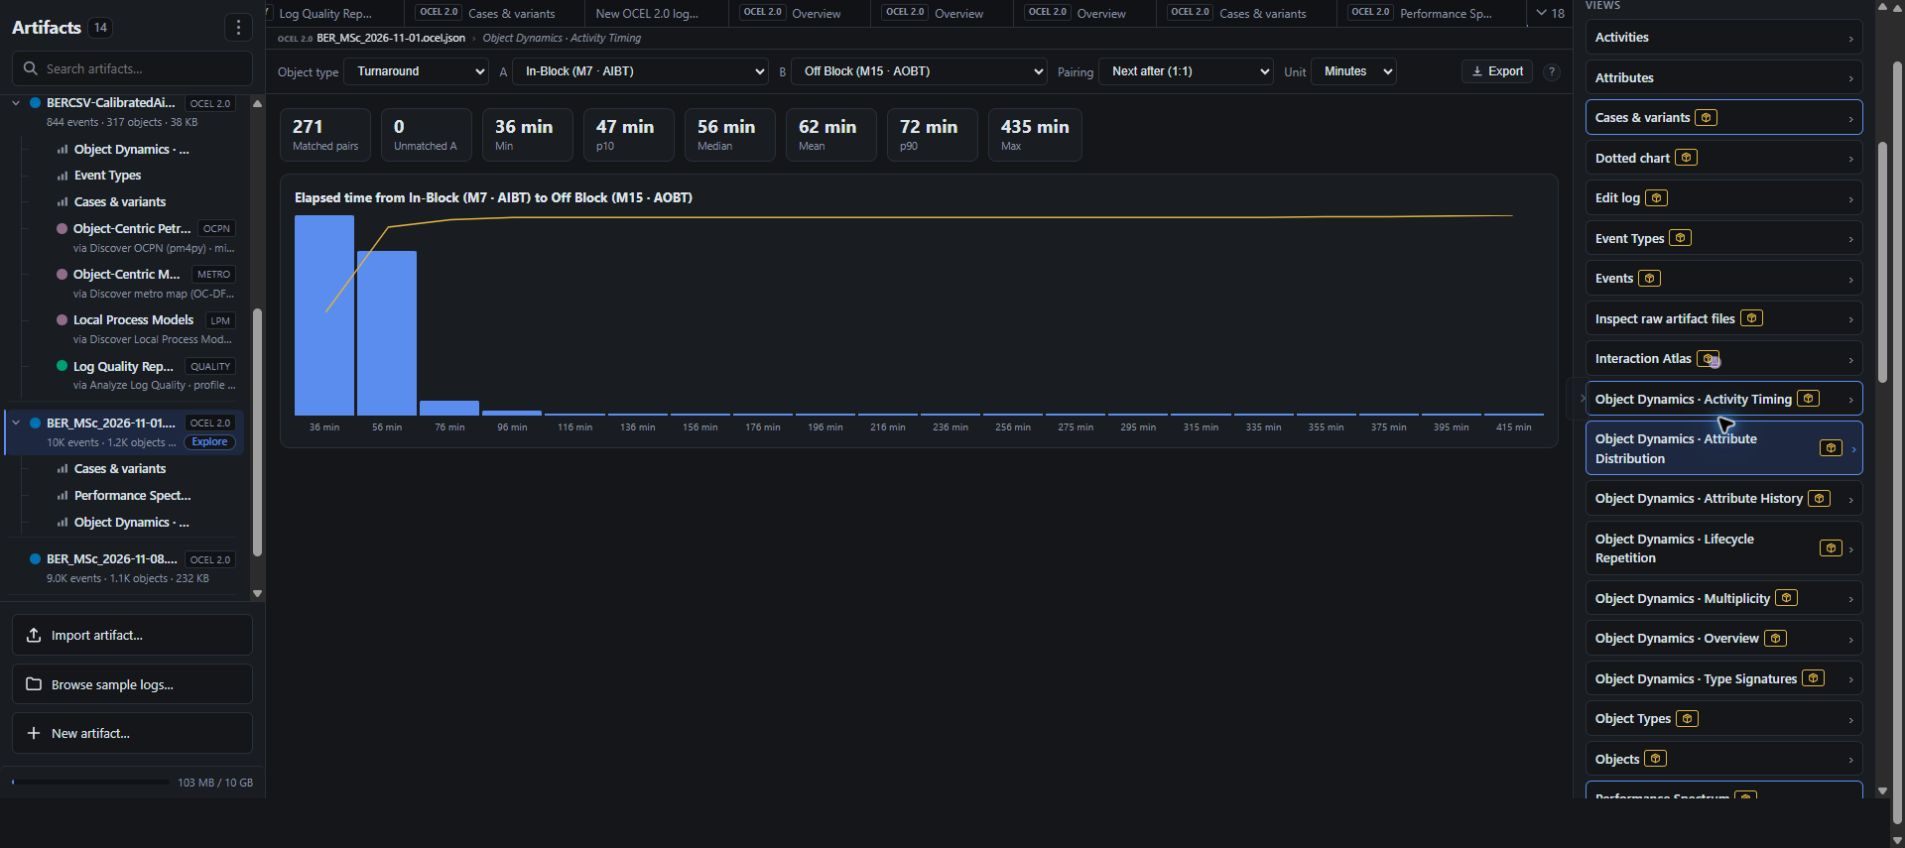
\includegraphics[width=\textwidth]{study_promenade_timing.jpg}
\caption{Promenade Object Dynamics/Activity Timing view of the 1 November literature-timing log. The data are generated simulation events.}\label{fig:promenade}
\end{figure}

\section{Resource queues and handling dependencies}
In the individual literature-timing runs, mean fuel-dispatch waiting is 3.785 minutes on 1 November and 1.255 minutes on 8 November. Cleaning-team waiting is 0.018 and approximately zero minutes; tug-allocation waiting is 0.033 and approximately zero. The 1 November 90th-percentile fuel waiting time is 14.20 minutes, with a maximum of 38.28 minutes.

Nevertheless, the cabin/boarding branch is last ready in 230 of 271 turnarounds (84.9\%) and 192 of 238 (80.7\%). Fuel is last in only 21 and 10 cases; baggage handling is last in 20 and 36. This result distinguishes local waiting from final readiness. An aircraft can wait for fuel while cabin work continues. Reducing that wait may therefore leave the final completion time almost unchanged. The branch counts describe what happened at the join in these runs; a controlled change is needed to assess its effect on overall duration.
\begin{figure}[htbp]\centering
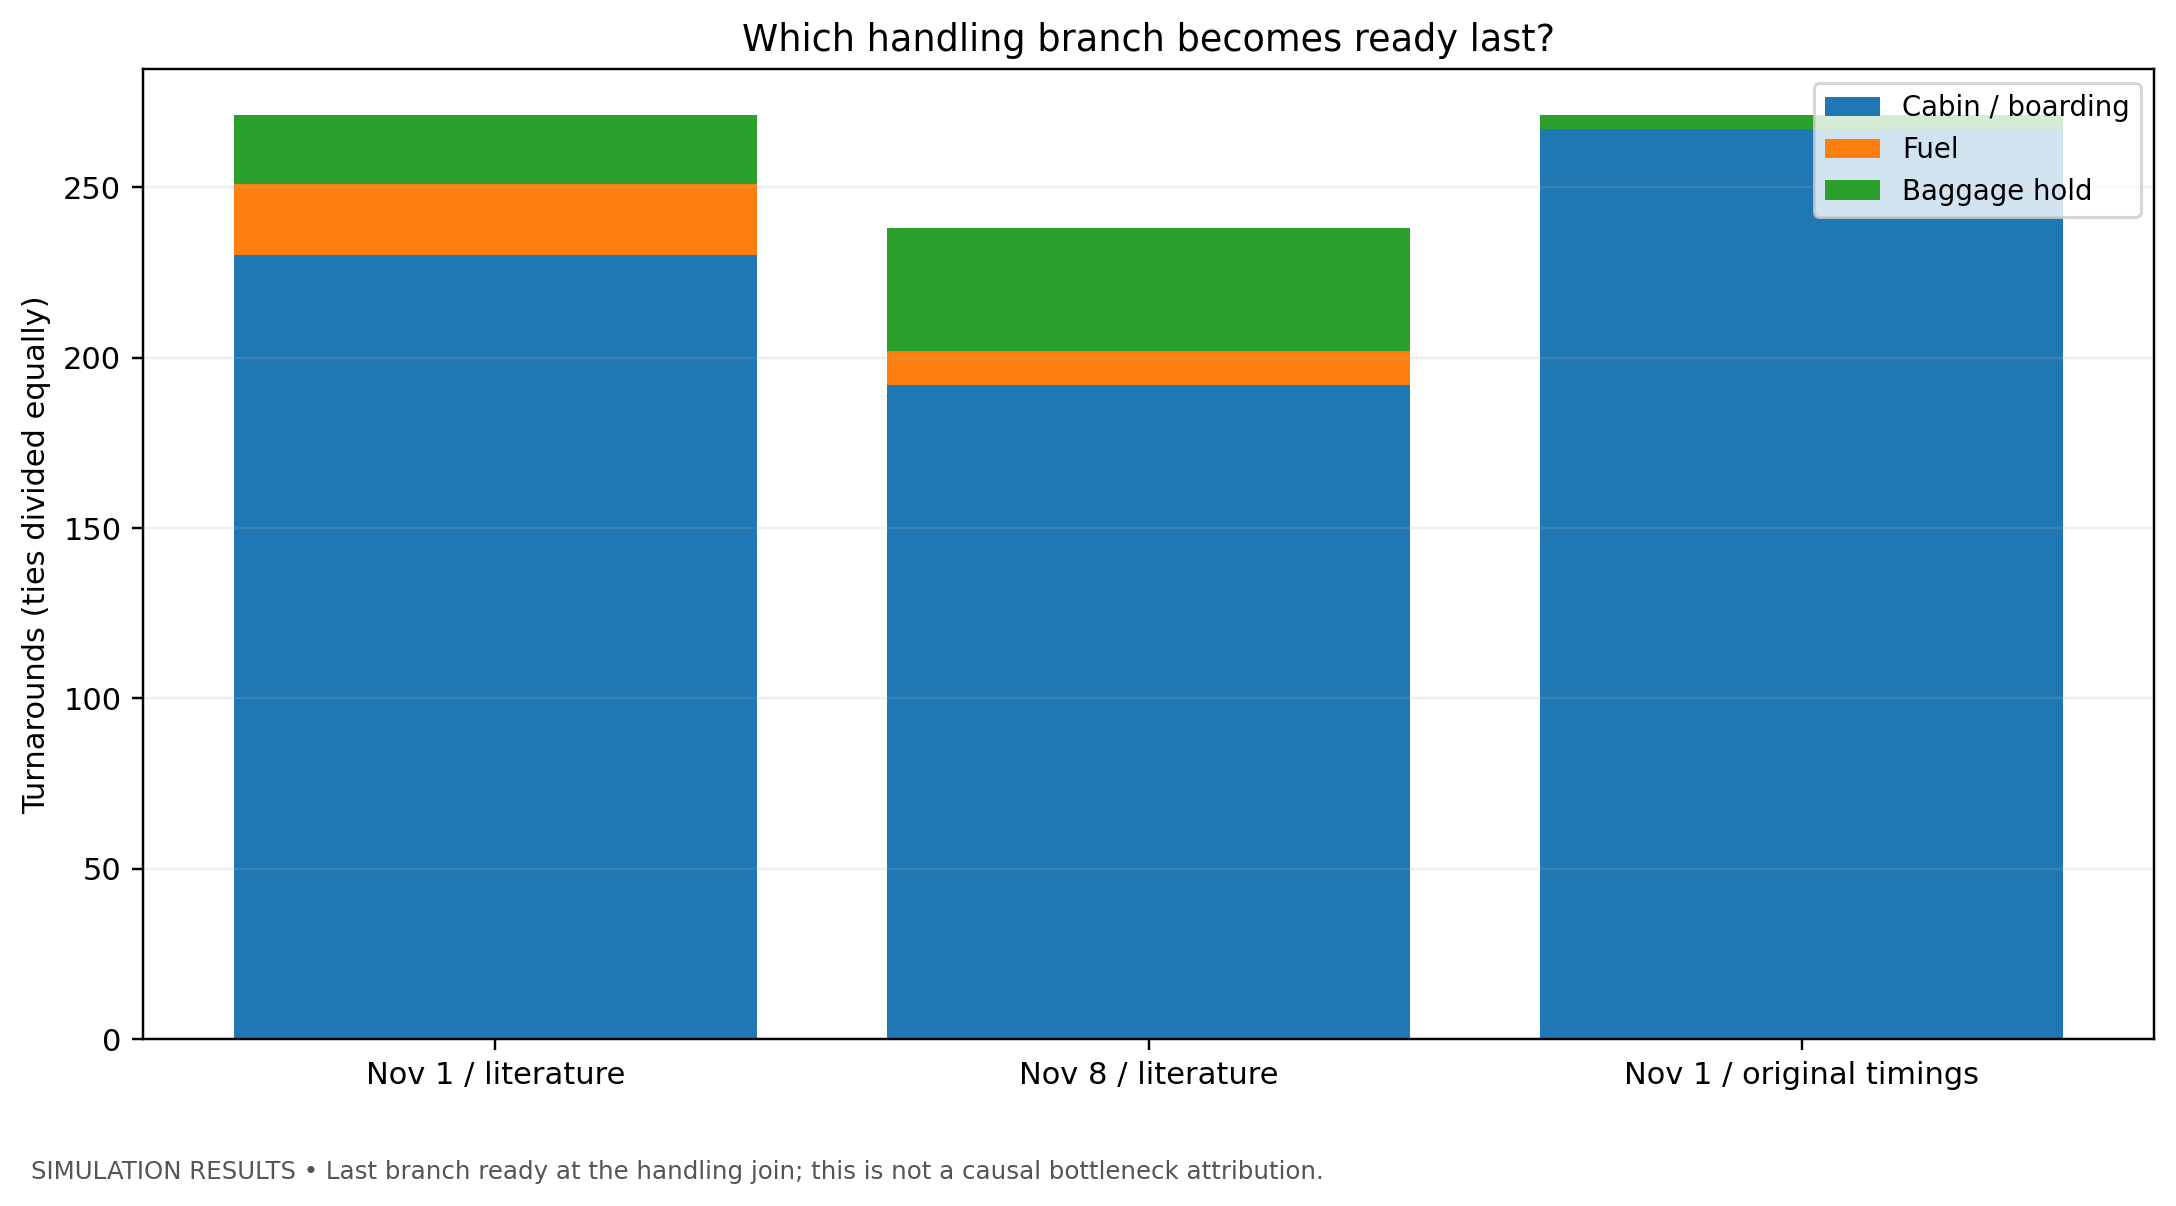
\includegraphics[width=\textwidth]{study_last_ready.png}
\caption{Last-ready handling branch in the original three simulation logs, calculated from output-token availability at the join. This supplementary Python figure uses exported events; it is not a Promenade-generated chart.}\label{fig:lastready}
\end{figure}

These observations partially address RQ2 by exposing parallel dependencies and resource contention within the simulation. They do not establish real terminal-versus-remote stand differences or quantify empirical inter-flight delay propagation. Workload counts per shared resource must also not be called time utilization without occupancy-duration calculations.

\section{Case-definition diagnostic}
The 1 November Promenade overview has two connected object components, with 94\% of objects in the largest. Reusable resources connect many rotations; a connected-component case definition would therefore merge most of the day. A leading Turnaround extraction returns 271 executions and 271 variants at the selected settings, but expanded executions can include shared-resource events. One expanded execution displays approximately 16.7 hours, which is not that turnaround's paired block duration. The analysis therefore uses direct paired milestones for duration statistics. A SQL-discovered object-centric directly-follows graph was produced; the separate metro-map layout was canceled after stalling and is not a completed result.

\section{Observed proxy discrepancies}
The first 1 November literature run has a simulated planned-arrival-to-takeoff proxy median of 79.63 minutes, close to the observed boundary-proxy median of 79.12. However, their means are 85.63 versus 156.17 minutes, with mean bias $-70.55$ minutes and mean absolute discrepancy 92.09 minutes. On 8 November, mean bias is $-101.60$ minutes and mean absolute discrepancy 116.00 minutes.
\begin{figure}[htbp]\centering
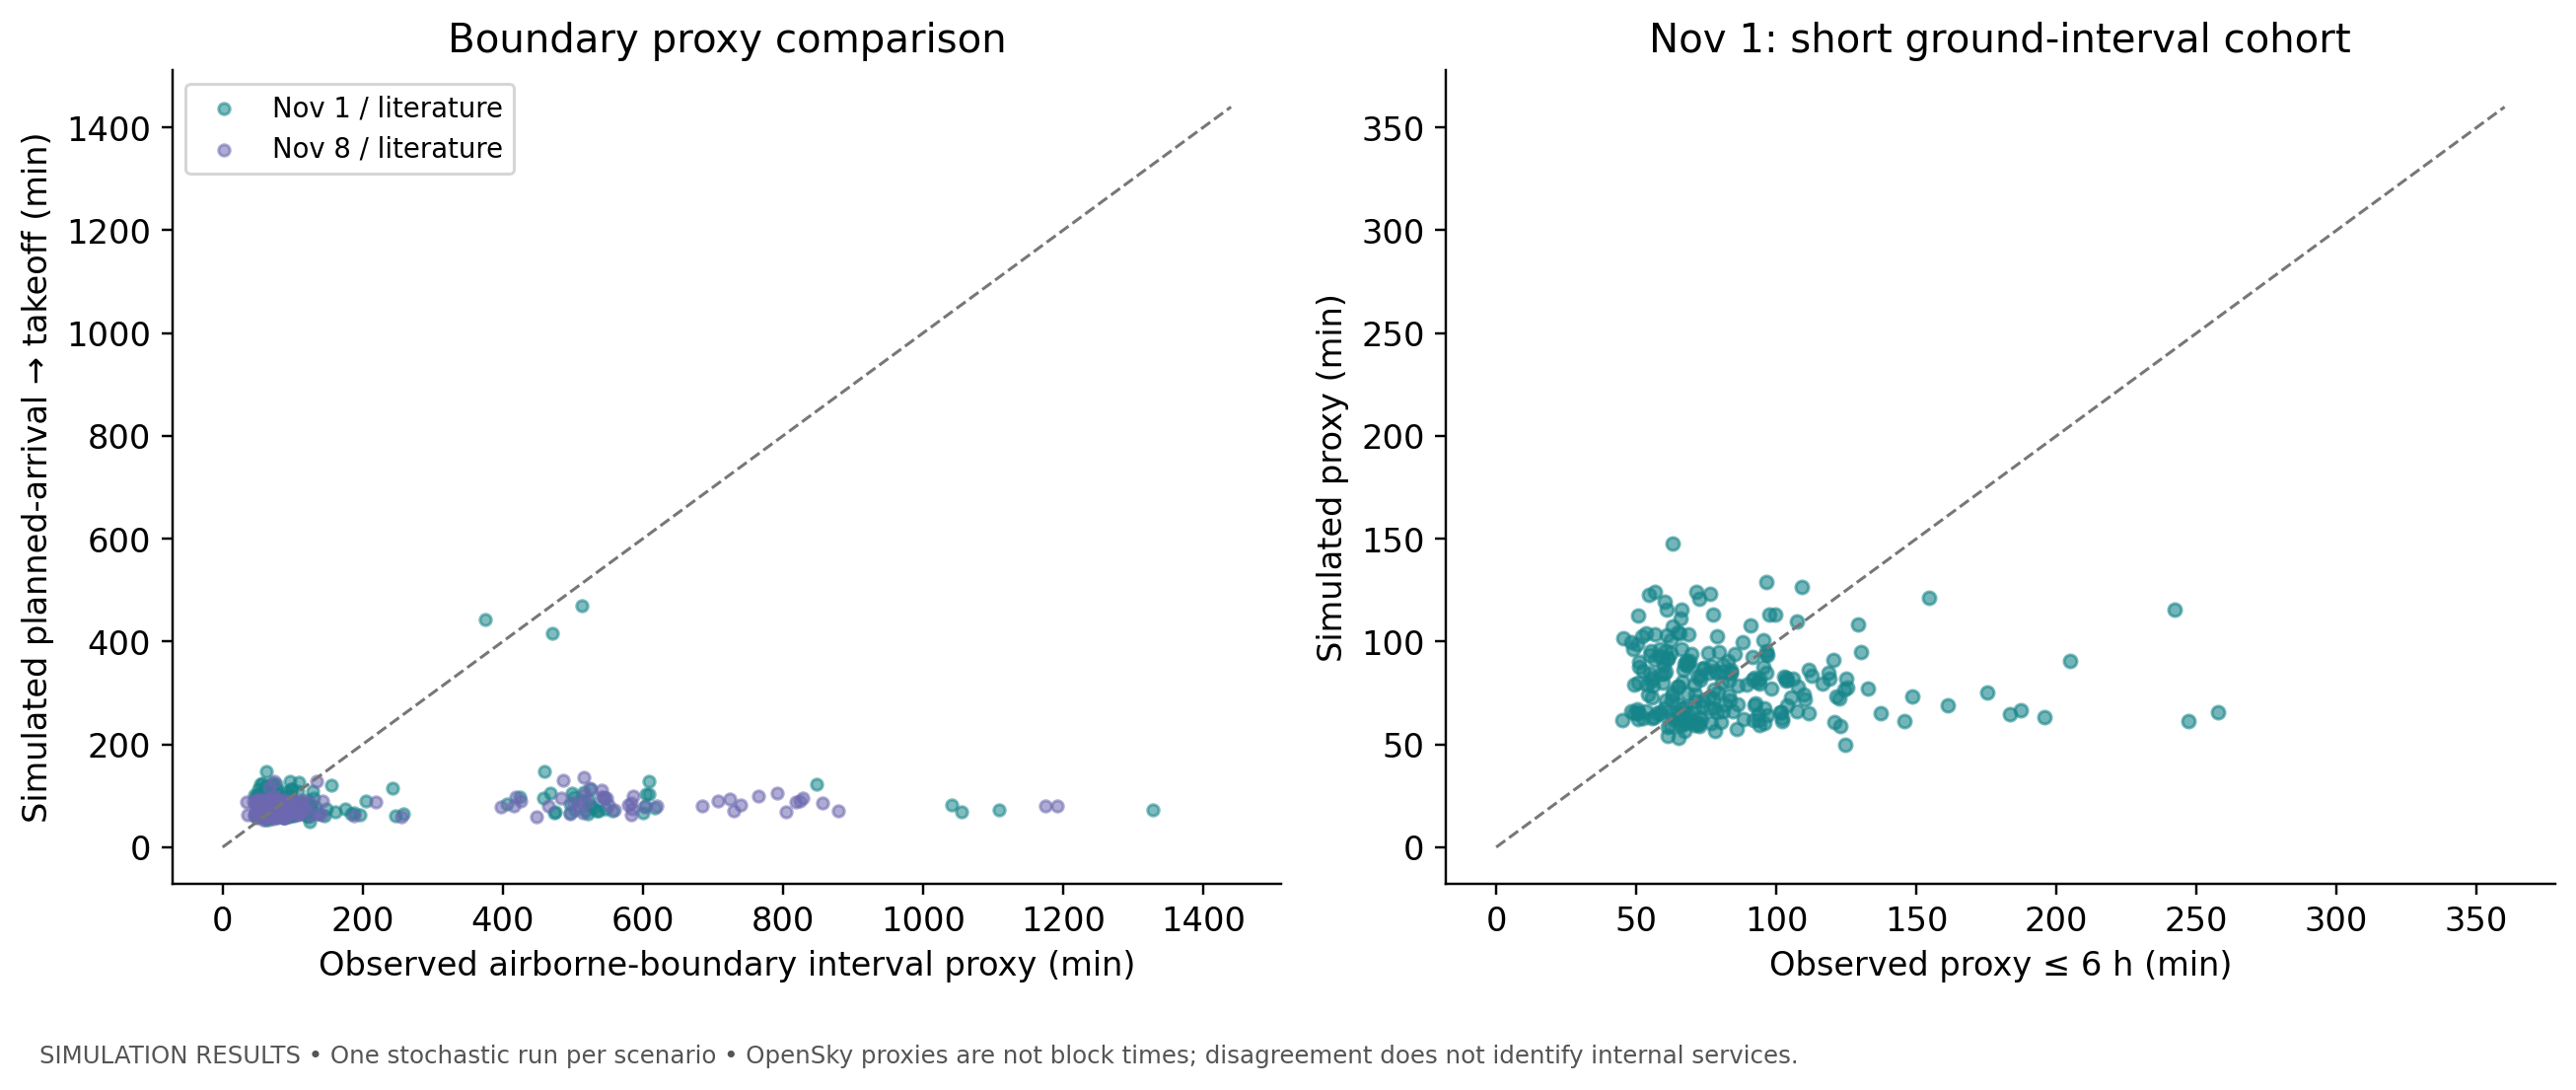
\includegraphics[width=\textwidth]{study_proxy_comparison.png}
\caption{Exploratory comparison with observed boundary proxies for the initial logs. These are not errors against measured AIBT--AOBT. Long stays and differing timestamp semantics limit interpretation.}\label{fig:proxy}
\end{figure}

The similar medians are therefore insufficient to demonstrate agreement. The much larger observed mean indicates a different distribution, particularly for long intervals. The simulator begins handling after arrival and departs when ready, whereas the observations can also contain parking and schedule buffers. Before fitting durations, we need to review the pairings, separate short and long stays, and represent departure scheduling where justified. Increasing cleaning or fueling time simply to match the total interval would not resolve these differences.

\section{Repeated timing and policy comparisons}
All 60 controlled runs complete and pass integrity checks. Table~\ref{tab:controlled} gives the mean of five replication means per date/scenario. Figure~\ref{fig:timing} shows the individual run means and intervals.
\begin{table}[htbp]\centering\small
\begin{tabular}{lrr}\hline
Scenario & Nov. 1 mean [95\% CI] & Nov. 8 mean [95\% CI]\\\hline
Original, inherited policy & 86.91 [84.83,89.00] & 72.73 [69.30,76.17]\\
Literature, inherited policy & 61.91 [59.82,64.01] & 59.22 [58.91,59.52]\\
Original, disabled curfew & 66.73 [66.14,67.32] & 66.07 [65.78,66.37]\\
Literature, disabled curfew & 59.20 [58.59,59.81] & 59.03 [58.45,59.61]\\
Six cleaning teams, disabled & 59.26 [58.39,60.13] & 59.20 [58.33,60.06]\\
Six+six fuel units, disabled & 58.58 [58.34,58.81] & 58.81 [58.56,59.06]\\\hline
\end{tabular}
\caption{Mean simulated block duration in minutes. Resource variants use literature timings; the reference has nine cleaning teams and four+four fuel units. Intervals quantify between-run simulation variability only.}\label{tab:controlled}
\end{table}
\begin{figure}[htbp]\centering
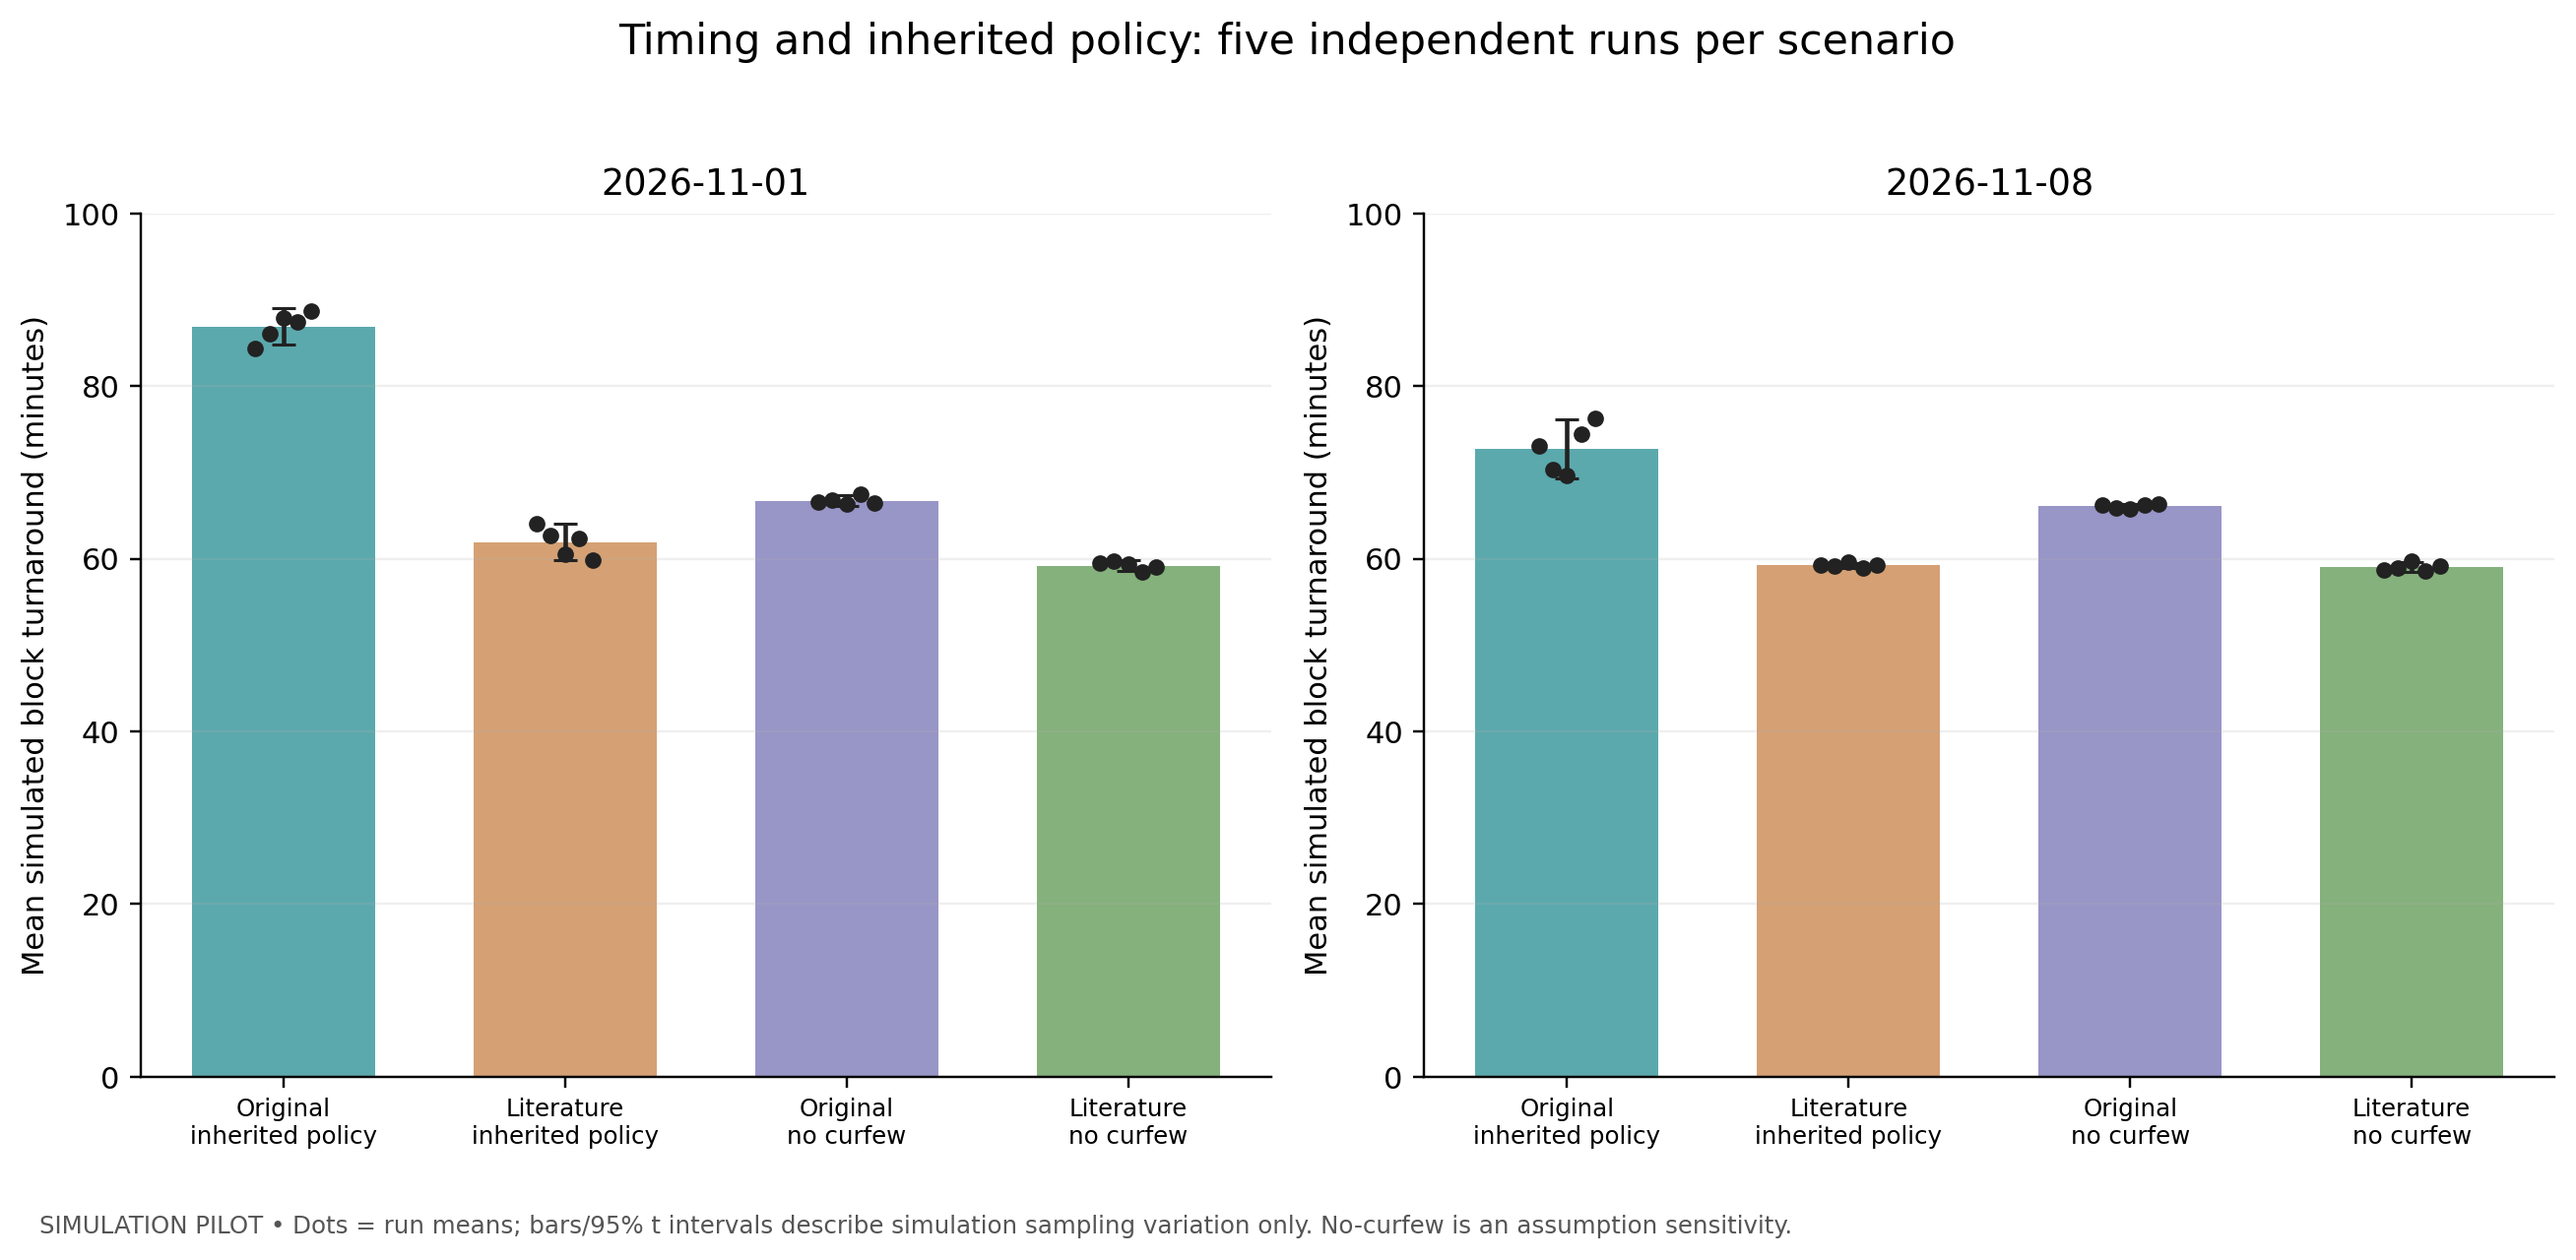
\includegraphics[width=\textwidth]{study_timing_policy.png}
\caption{Timing/policy comparisons: five independent run means per scenario, with Student-$t$ 95\% intervals. Disabled curfew is a diagnostic assumption sensitivity.}\label{fig:timing}
\end{figure}

With curfew disabled, literature-minus-original timing differences are $-7.53$ minutes on 1 November (Welch 95\% CI $[-8.24,-6.82]$) and $-7.04$ on 8 November ($[-7.62,-6.47]$). Under inherited policy the differences increase to $-25.00$ ($[-27.45,-22.54]$) and $-13.52$ ($[-16.94,-10.09]$). The timing difference is therefore substantially larger when the inherited policy is active. This shows that timing and policy interact in the model. It does not show that the transferred service durations are more accurate than the original functions.

An additional exploratory interaction contrast, added while inspecting the pilot, subtracts the disabled-curfew timing difference from the inherited-policy timing difference. Estimates are $-17.46$ minutes ($[-19.96,-14.97]$) and $-6.48$ ($[-9.88,-3.08]$). This is a conditional model finding, not a preregistered confirmatory result or a causal statement about airport regulations.

\section{Repeated resource sensitivity}
Under literature timings and disabled curfew, increasing fueling capacity from eight to twelve units reduces mean dispatch waiting from 3.042 to 0.168 minutes on 1 November and from 2.040 to 0.066 on 8 November. Final block-duration differences are much smaller: $-0.62$ minutes (95\% CI $[-1.23,-0.02]$) and $-0.22$ ($[-0.79,0.35]$). The November 8 interval includes zero, so this pilot does not clearly resolve the direction of that overall difference. Taken together, the results show a large reduction in the local fuel queue and a much smaller change in final turnaround. These are different outcomes and should be reported separately.
\begin{figure}[htbp]\centering
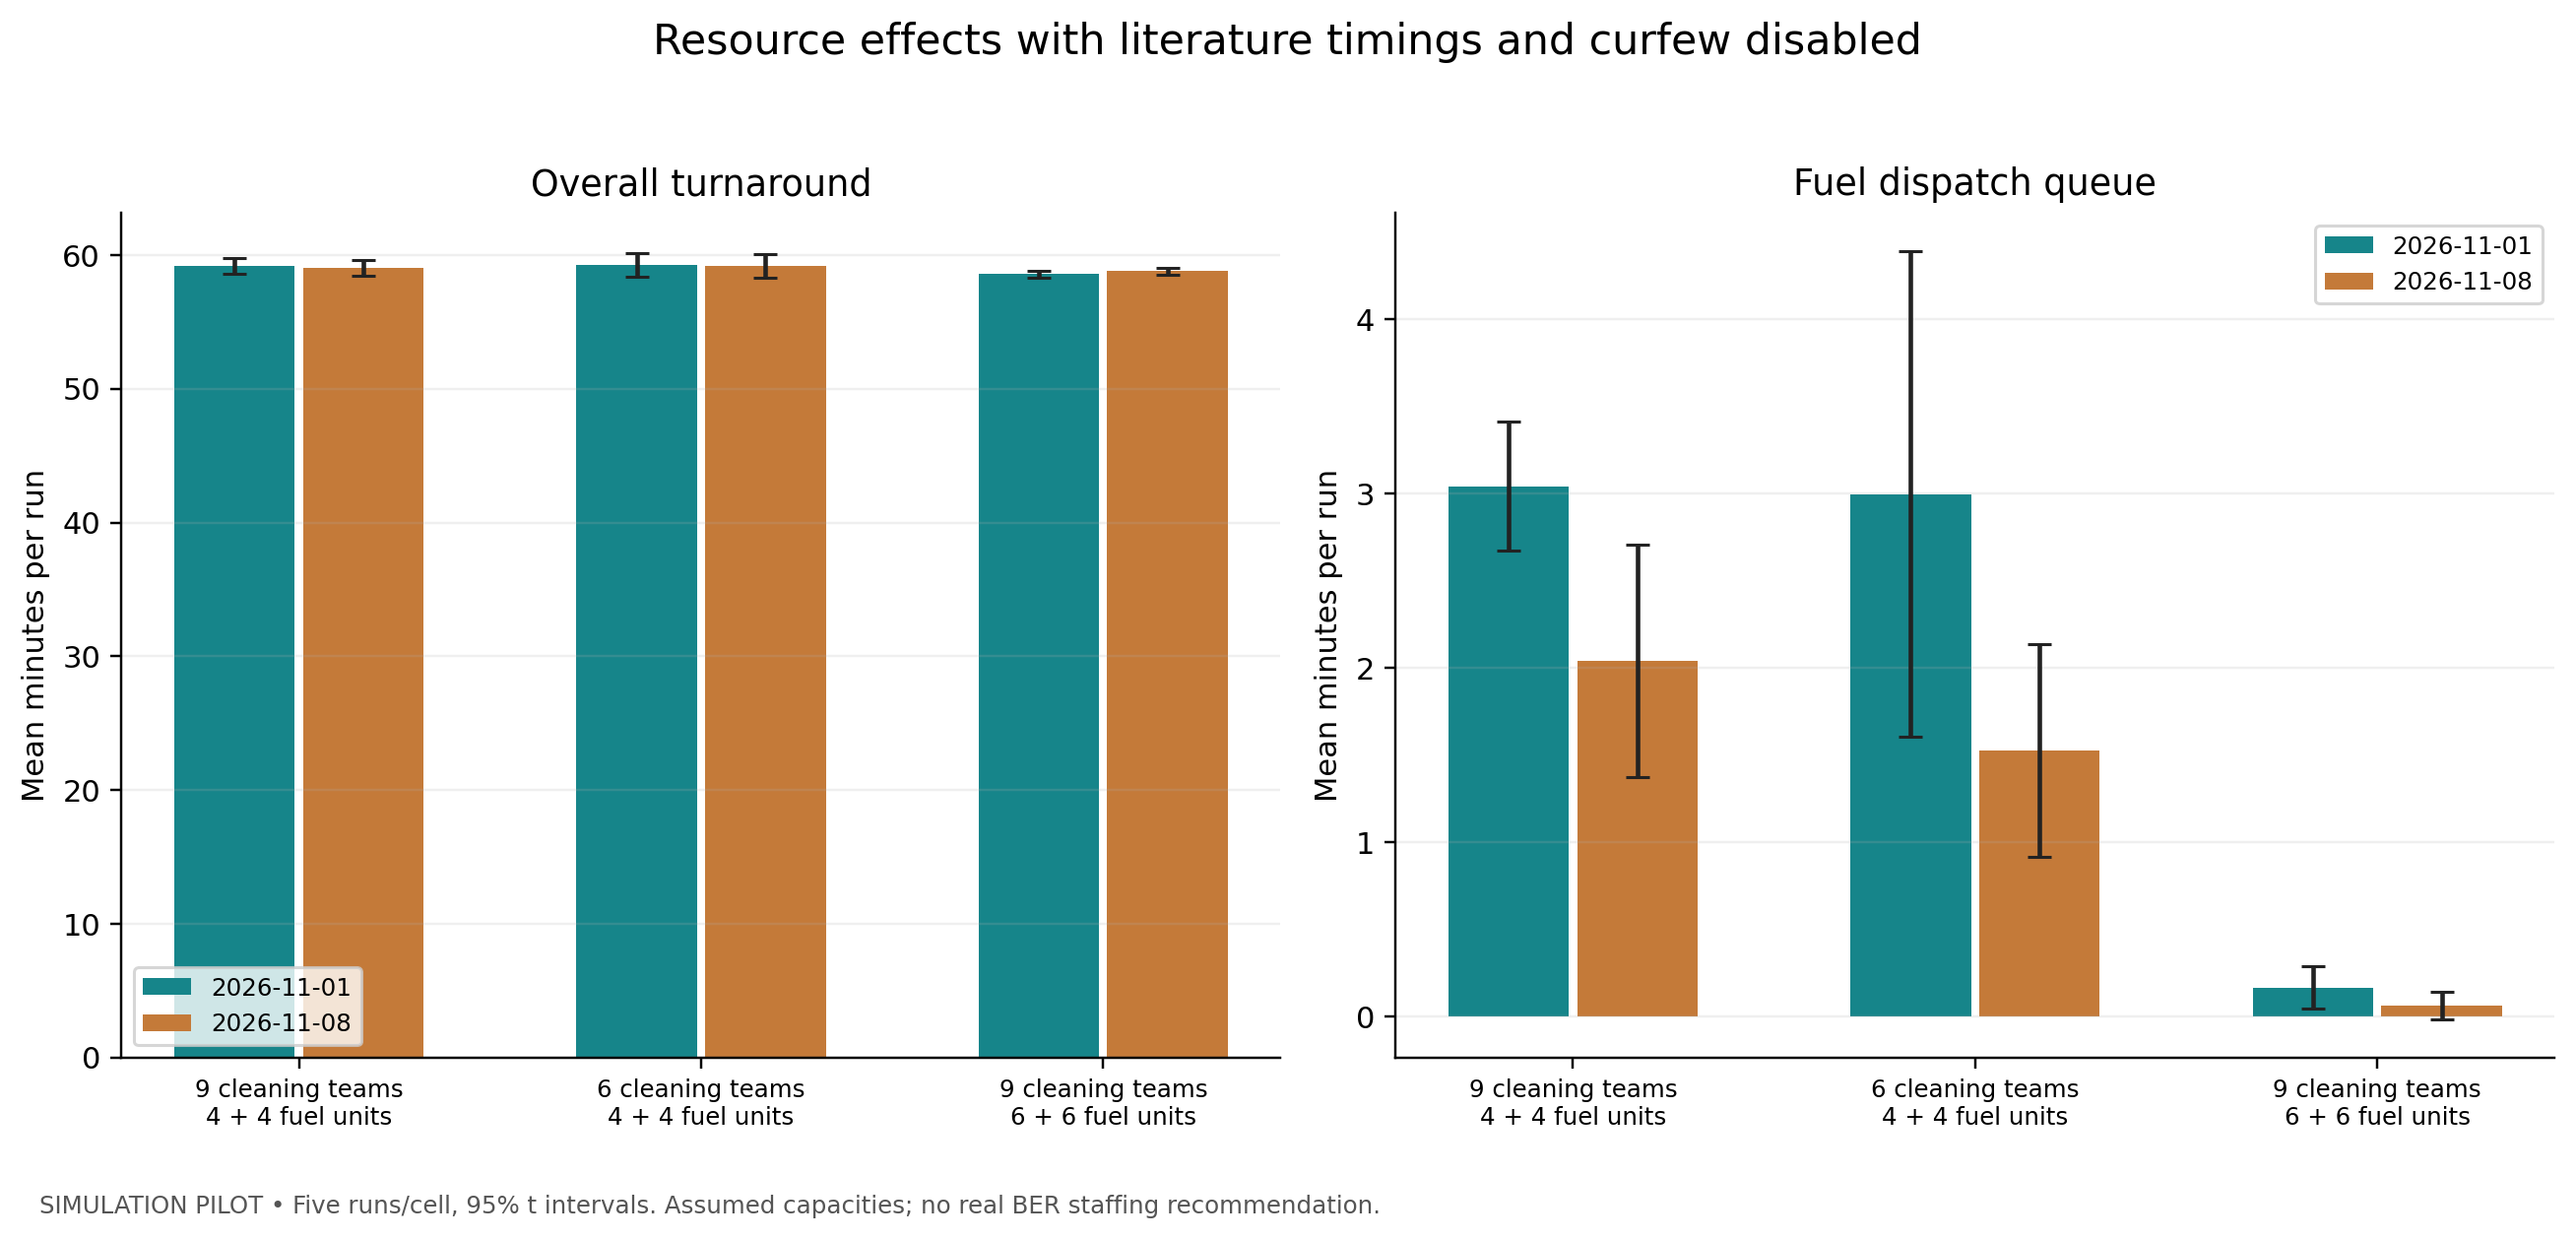
\includegraphics[width=\textwidth]{study_resource_sensitivity.png}
\caption{Resource sensitivity: overall turnaround and fuel-dispatch waiting respond differently. Counts are assumed model capacities, not verified BER staffing.}\label{fig:resource}
\end{figure}

Reducing cleaning teams from nine to six produces estimated block-duration increases of 0.07 minutes ($[-0.84,0.97]$) and 0.17 ($[-0.72,1.05]$). Both intervals include zero. The experiment therefore does not provide a clear direction for the change in block duration. This result does not prove that six and nine teams are equivalent, and it does not provide a basis for reducing staffing at BER.
\begin{figure}[htbp]\centering
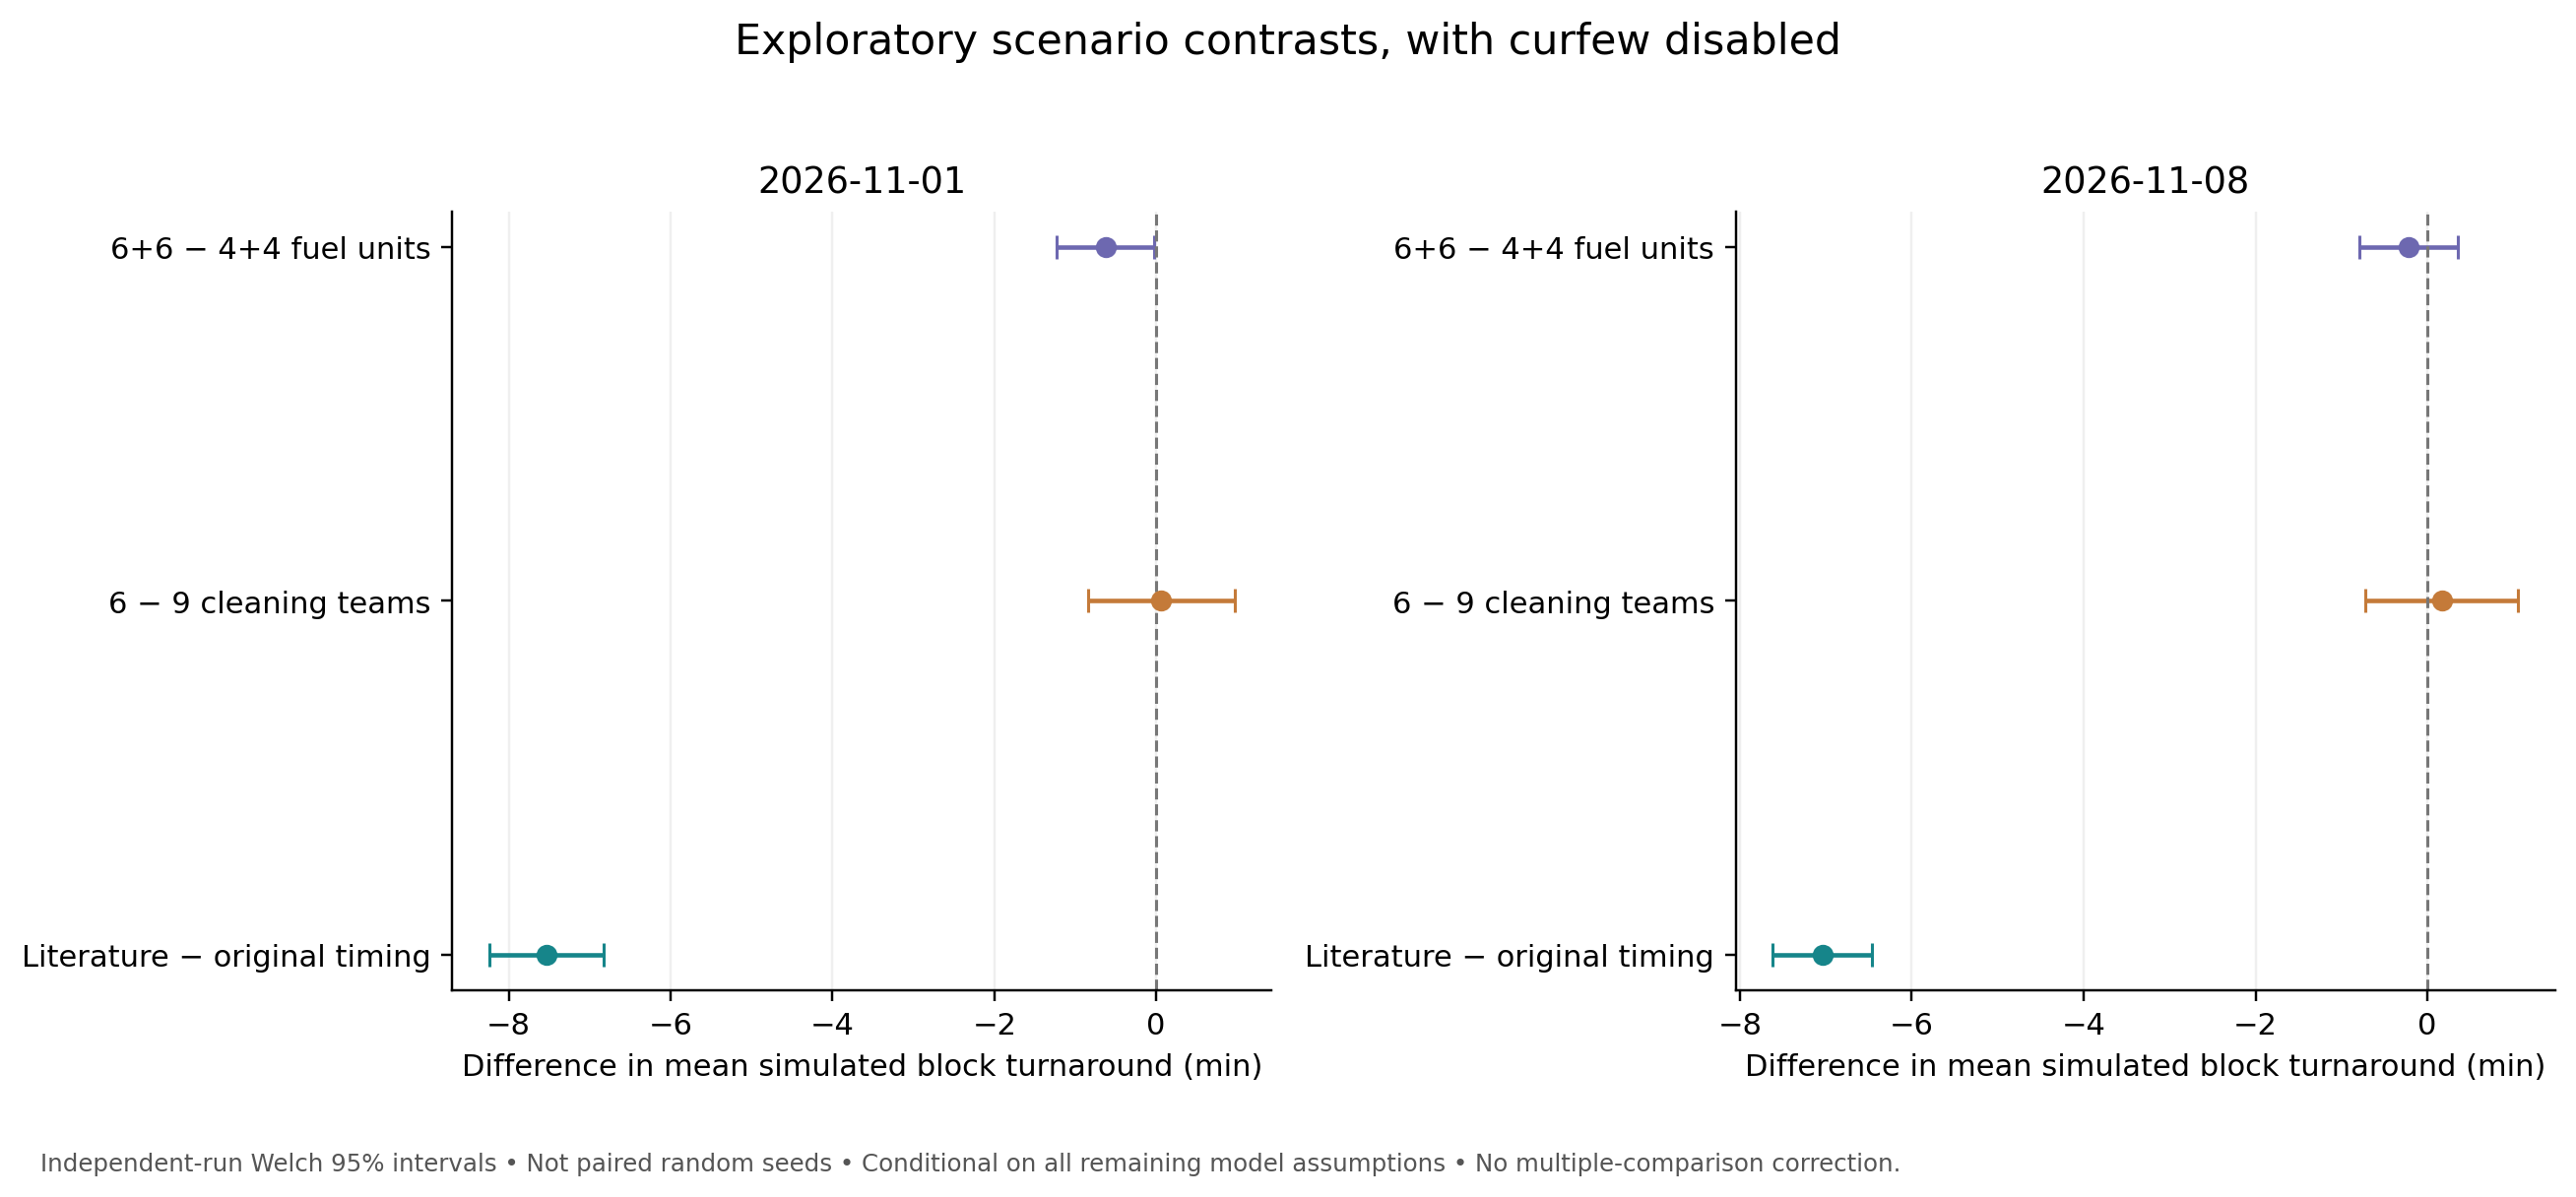
\includegraphics[width=\textwidth]{study_contrasts.png}
\caption{Exploratory independent-run Welch 95\% intervals for block-duration differences with curfew disabled. No multiplicity adjustment is applied.}\label{fig:contrasts}
\end{figure}

For RQ3, these scenarios demonstrate a functioning evaluation method and conditional trade-offs. They do not establish a cost-optimal configuration, compare alternative dispatch priorities, or optimize real BER resource allocation.


\section{Summary}
The initial analysis identifies fuel-dispatch queues, frequent last-ready cabin branches and important limitations in the interpretation of extracted executions. The repeated experiment then shows that policy logic changes the apparent effect of service timings. Increasing fuel capacity greatly reduces dispatch waiting, but its effect on final turnaround is much smaller. These findings support conditional analysis of the modeled system; they do not yet establish empirical calibration or an optimal resource configuration.

\cleardoublepage
\chapter{Discussion and Threats to Validity}
\label{ch:discussion}

This chapter explains what the results contribute to the research questions. We then discuss the inherited policy and the main limitations of the data, model and analysis. The aim is to distinguish findings supported by the experiment from conclusions that still require further observations or experiments.

\section{Answers supported by the current evidence}
\subsection{RQ1: data-informed calibration}
The collected observations support a finite arrival schedule, candidate aircraft pairings and checks on selected flight attributes. They do not provide enough information to estimate cleaning, fueling or boarding durations separately. Several activities and waiting periods can occur within the same boundary interval. We can therefore use the data to construct demand, but the internal services still require literature inputs and assumptions. Service start/end records, passenger counts and reliable block timestamps would be needed for stronger activity-level calibration.

\subsection{RQ2: dependencies, queues and propagation}
Object-linked logs show how shared resource availability and parallel branches contribute to simulated waiting and readiness. Fuel dispatch has the clearest local queue in the initial runs, yet cabin/boarding is usually the final handling branch. The capacity intervention supports the interpretation that removing fuel waiting can have limited effect on final completion because work overlaps.

The answer to RQ2 remains partial. Aircraft identities and reusable resources allow contention across turnarounds, but we have not measured how an imposed delay passes from one flight to another. We also have not isolated differences between terminal and remote stands. Such a comparison requires reliable stand classifications and explicit assumptions for bus and access time. It must also control the demand and initial resource state so that the source of a difference can be explained.

\subsection{RQ3: conditional resource evaluation}
Repeated capacity comparisons demonstrate how to evaluate local queues alongside overall turnaround and uncertainty. The findings favor reporting both levels rather than selecting a configuration using queue length alone. However, only two capacity alternatives were tested, with assumed resources and no cost objective. The current evidence cannot establish an optimal resource configuration or real staffing recommendation.

\section{Policy and clock semantics}
BER's official guidance describes a core night-flight restriction from 00:00 to 05:00 and constraints in the adjacent 23:00--24:00 and 05:00--06:00 windows \cite{ber_night}. The inherited model instead applies its helper before pre-boarding and pushback clearance. Those applications do not constitute a complete operational movement-eligibility model.

The installed CPNsim runtime was probed at epoch \texttt{2026-11-01T00:00:00Z}: its hour helper returns zero, while Berlin local hour is one. Engine source also uses UTC \cite{cpnsim}. Thus the inherited 00:00--05:00 condition corresponds to 01:00--06:00 local time on both study dates. This mismatch is confirmed, rather than a possible explanation inferred solely from plotted tails.

The controlled experiment deliberately retains the inherited implementation in its policy cells and disables the entire helper in the diagnostic cells. Neither is presented as a verified BER replacement. A subsequent version must use Europe/Berlin time, including daylight-saving changes across the full collection, and distinguish movement restrictions, shoulder windows, exceptions and independent cabin work. The present analysis does not make a legal-compliance determination.

\section{Data and construct validity}
ICAO24 adjacency provides candidate rotations rather than certified ground movements. Missing flights, airport-estimation errors or identifier issues may affect pairing. OpenSky observation boundaries and simulated block milestones are different constructs. A-CDM reference matches and a timezone hypothesis do not remove these differences. The observed-proxy discrepancies should therefore be reported without calling them block-time prediction errors.

Long stays, planned departure buffers and overnight parking are not modeled. The selected cohort also omits competing traffic, and every daily run begins with free resources. These choices can materially alter queues. Fictitious geometry, passenger load, PRM demand, carrier class, optional services and non-narrowbody functions further restrict transfer to real BER operations.

\section{Statistical and analytical validity}
The confidence intervals describe variation across five replications under fixed model assumptions. They do not include uncertainty in passenger loads, capacities or the process structure. The runs are unpaired because the runtime does not expose seed control. Repeating the procedure will therefore generate new stochastic outputs. We also report several exploratory comparisons without a multiple-comparison adjustment. An interval containing zero is not proof of no effect, while an interval that only narrowly excludes zero should be interpreted cautiously.

The timing comparison changes cleaning, fueling and boarding together. It therefore cannot determine which individual service explains the difference. It also cannot separate the effect of a changed mean duration from that of changed variability. November 8 is a later-date scenario with no outcome-based tuning in this pilot, but is not a completed held-out predictive validation. Formal empirical conformance, contact/remote stratification, resource time utilization, cost analysis and external replication remain incomplete.

The scope of an extracted execution also affects interpretation. A shared resource connects several rotations, so an expanded graph can include events outside the focal turnaround. We use one-to-one milestone pairs to calculate block duration and inspect the graph separately. This prevents a long expanded execution from being reported as a measured turnaround interval.

\section{Relation to the Trace-Reconstruction Study}
Tkacenko's evaluation shows that traces selected using total turnaround boundaries can still disagree with observed internal activity durations \cite[Section~6.2]{tkacenko2026}. Our results identify a related limitation from another direction: a simulated median close to an observed proxy median can coexist with a large mean discrepancy. In both cases, an aggregate duration provides only limited evidence about the internal process.

The evaluation settings are different. Tkacenko uses limited activity-level ground truth and temporal acceptance filtering, whereas our current Berlin analysis has no comparable internal service observations. Her state-space checks also concern a time-neutralized model abstraction. Our completed-run checks do not reproduce that analysis or establish the same properties. Keeping these differences explicit avoids transferring validation claims between studies.

\section{Remaining Work Before Stronger Conclusions}
The next model version should correct local-time movement policy, resolve aircraft-type candidates and distinguish operational turnarounds from long stays. Evaluation should then use independently selected dates and matching observable quantities, without forcing observed departures. RQ2 additionally requires terminal/remote stratification and controlled delay-propagation experiments. RQ3 needs broader input/capacity sensitivity and a declared operational or cost objective. These tasks should precede claims of validated calibration or optimal allocation.


\section{Summary}
The completed pilot provides evidence about dependencies and assumption sensitivity within the adapted model. Its main limits concern missing service observations, incomplete operational context and the inherited policy. Further work should address these limits before extending the findings to actual BER operations. The distinction between technical completion and empirical validity remains central to that evaluation.

\cleardoublepage
\chapter{Conclusion}
\label{ch:conclusion}

Aircraft turnaround involves concurrent activities and shared resources, but the available observations describe only part of this process. This thesis examines how those observations can support an object-centric simulation while keeping missing information explicit. We adapt the supplied extended airport model, prepare daily Berlin inputs and analyze the generated logs in Promenade.

For RQ1, the work demonstrates how to construct finite demand from candidate aircraft-linked intervals and retain the source and meaning of each input. It also identifies the limit of the available data: internal service durations cannot be recovered from the current boundary proxies alone. Literature-based timing functions therefore remain assumptions rather than fitted BER estimates.

For RQ2, the analysis shows how local waiting and parallel completion can lead to different conclusions. Fuel dispatch has a visible queue, while cabin and boarding work are usually last ready at the handling join. Shared-resource relationships also show why an expanded object-centric execution should not automatically be treated as one turnaround interval. A controlled terminal-versus-remote comparison and a quantified delay-propagation experiment remain incomplete.

For RQ3, the controlled pilot compares six scenarios on two dates with five runs per scenario and date. All 60 runs complete, producing 15,270 simulated executions from 509 reused empirical interval cases. With the inherited curfew helper disabled, literature timings shorten mean simulated block duration by 7.53 and 7.04 minutes. Increasing fuel capacity greatly reduces dispatch waiting, while the corresponding overall changes are only 0.62 and 0.22 minutes. These results demonstrate a method for conditional resource evaluation, rather than an optimal actual staffing configuration.

The policy comparison also reveals a confirmed UTC/local-time mismatch and a strong interaction between timing assumptions and inherited policy. This finding limits the interpretation of earlier differences and identifies a concrete requirement for the next model version.

\section{Future Work}
The next steps are to correct the local-time movement policy, separate operational turnarounds from long stays and resolve conflicting aircraft-type candidates. Empirical evaluation should then compare quantities with matching timestamp definitions on independently selected dates. Stand-specific and delay-propagation experiments are needed to complete RQ2, while broader uncertainty analysis and a declared allocation objective are needed for stronger RQ3 conclusions.

The completed work provides a traceable simulation and analysis procedure under limited observations. Its findings are useful for examining the modeled system and identifying assumptions that require further investigation. They do not yet establish a validated representation of BER ground handling.

\cleardoublepage
\chapter*{\acklabel}
\addcontentsline{toc}{chapter}{\acklabel}
I thank my supervisor, Istv\'an Koren, for providing the original extended airport model and guiding the research direction. The distinction between that baseline and the study modifications is maintained throughout this thesis.
\cleardoublepage
\appendix
\chapter{Reproducibility and artifact inventory}
\label{app:repro}
The original model is retained as \texttt{airport-extended.ocpn}; its SHA-256 is
\begin{quote}\footnotesize\texttt{b83e78fbdaa2289c406e359cffc080935b}\\
\texttt{d3ba586bae2f6a1858c77fa8f379d2}.\end{quote}
The two displayed lines form one continuous hash. The source attribution and MIT license accompanying the Studio-derived material are retained with the model package.

The prepared core input is \texttt{ber\_ground\_intervals\_core\_proxy.csv}. Daily case CSVs and manifests retain source keys and model assumptions. Version 2.0 daily OCEL exports and Promenade analysis are separate from version 2.1 controlled replications.

The controlled-study archive contains twelve built models, case CSVs/manifests, a frozen experiment plan, sixty per-case result files and corresponding summaries, replication metrics, scenario summaries, contrasts, validation results and three figures. Scripts implement model building, official-runtime execution and replication-level aggregation. Python dependencies are NumPy, pandas, SciPy and Matplotlib. Node.js and \texttt{@rwth-pads/cpnsim} 0.6.2 provide simulation execution. The runtime and full upstream raw collection are not bundled in that archive; absolute plan paths require adjustment after relocation.

The Promenade folder contains actual application captures/exports and supplementary Python figures, identified separately in captions. It also contains paired case metrics and analysis notes. The controlled replications are headless results, not sixty additional completed Promenade imports.

All reported controlled runs passed completion, case uniqueness, aircraft/resource-return and model-hash checks. These are technical integrity checks, distinct from official OCEL schema validation, process conformance or empirical accuracy. The 10,940-case model is load-tested only. Random-seed control is unavailable, so repeating the procedure will produce new stochastic outputs.

\cleardoublepage
\phantomsection
\addcontentsline{toc}{chapter}{\biblabel}
\printbibliography[title=\biblabel]
\cleardoublepage
\listoffigures
\cleardoublepage
\listoftables
\end{document}
